\section{Memristors}
\label{sec:memristors}

Memristors are the lesser known fourth fundamental passive component of electronics, among resistors, capacitors and inductor.
It was first theorized in 1971 by L. Chua from UC Berkeley, in \cite{TheoMemristor}. The name comes from the blend of \textit{memory} and \textit{resistance}.
The theory behind the component was extracted from a missing component to link the fundamental circuit variables. In figure \ref{fig:fundComp}, the four fundamental variables are on each side of the square, with the ones on opposite sides being linked as shown in the following equations :
\begin{equation}
  d\phi = v\cdot dt
\end{equation}

\begin{equation}
  dq = i\cdot dt
\end{equation}
Resistors, capacitors and inductors were already discovered and well known, so it was theorized that a fourth device should then exists to physically link flux ($\phi$) and charge ($q$).  The flux in this case is not a magnetic flux and is defined as such : $ d\phi=V\cdot dt \implies \phi =  \int V(t) \,dt  $.\\
The component stayed theoretical until 2008 when it's been implemented in a physical device for the first time \cite{Strukov2008}. It took 37 years to actually have a working device.\\
There is then an extention of this theoretical device to another, the memristive device. It was theorized in 1976 by L. Chua and S. M. Kang \cite{memrestiveDev}. The difference between the memristor and the memristive device is its internal behavior. Memristive device are commonly referred to as memristor as well.

\begin{figure}[H]
  \centering
  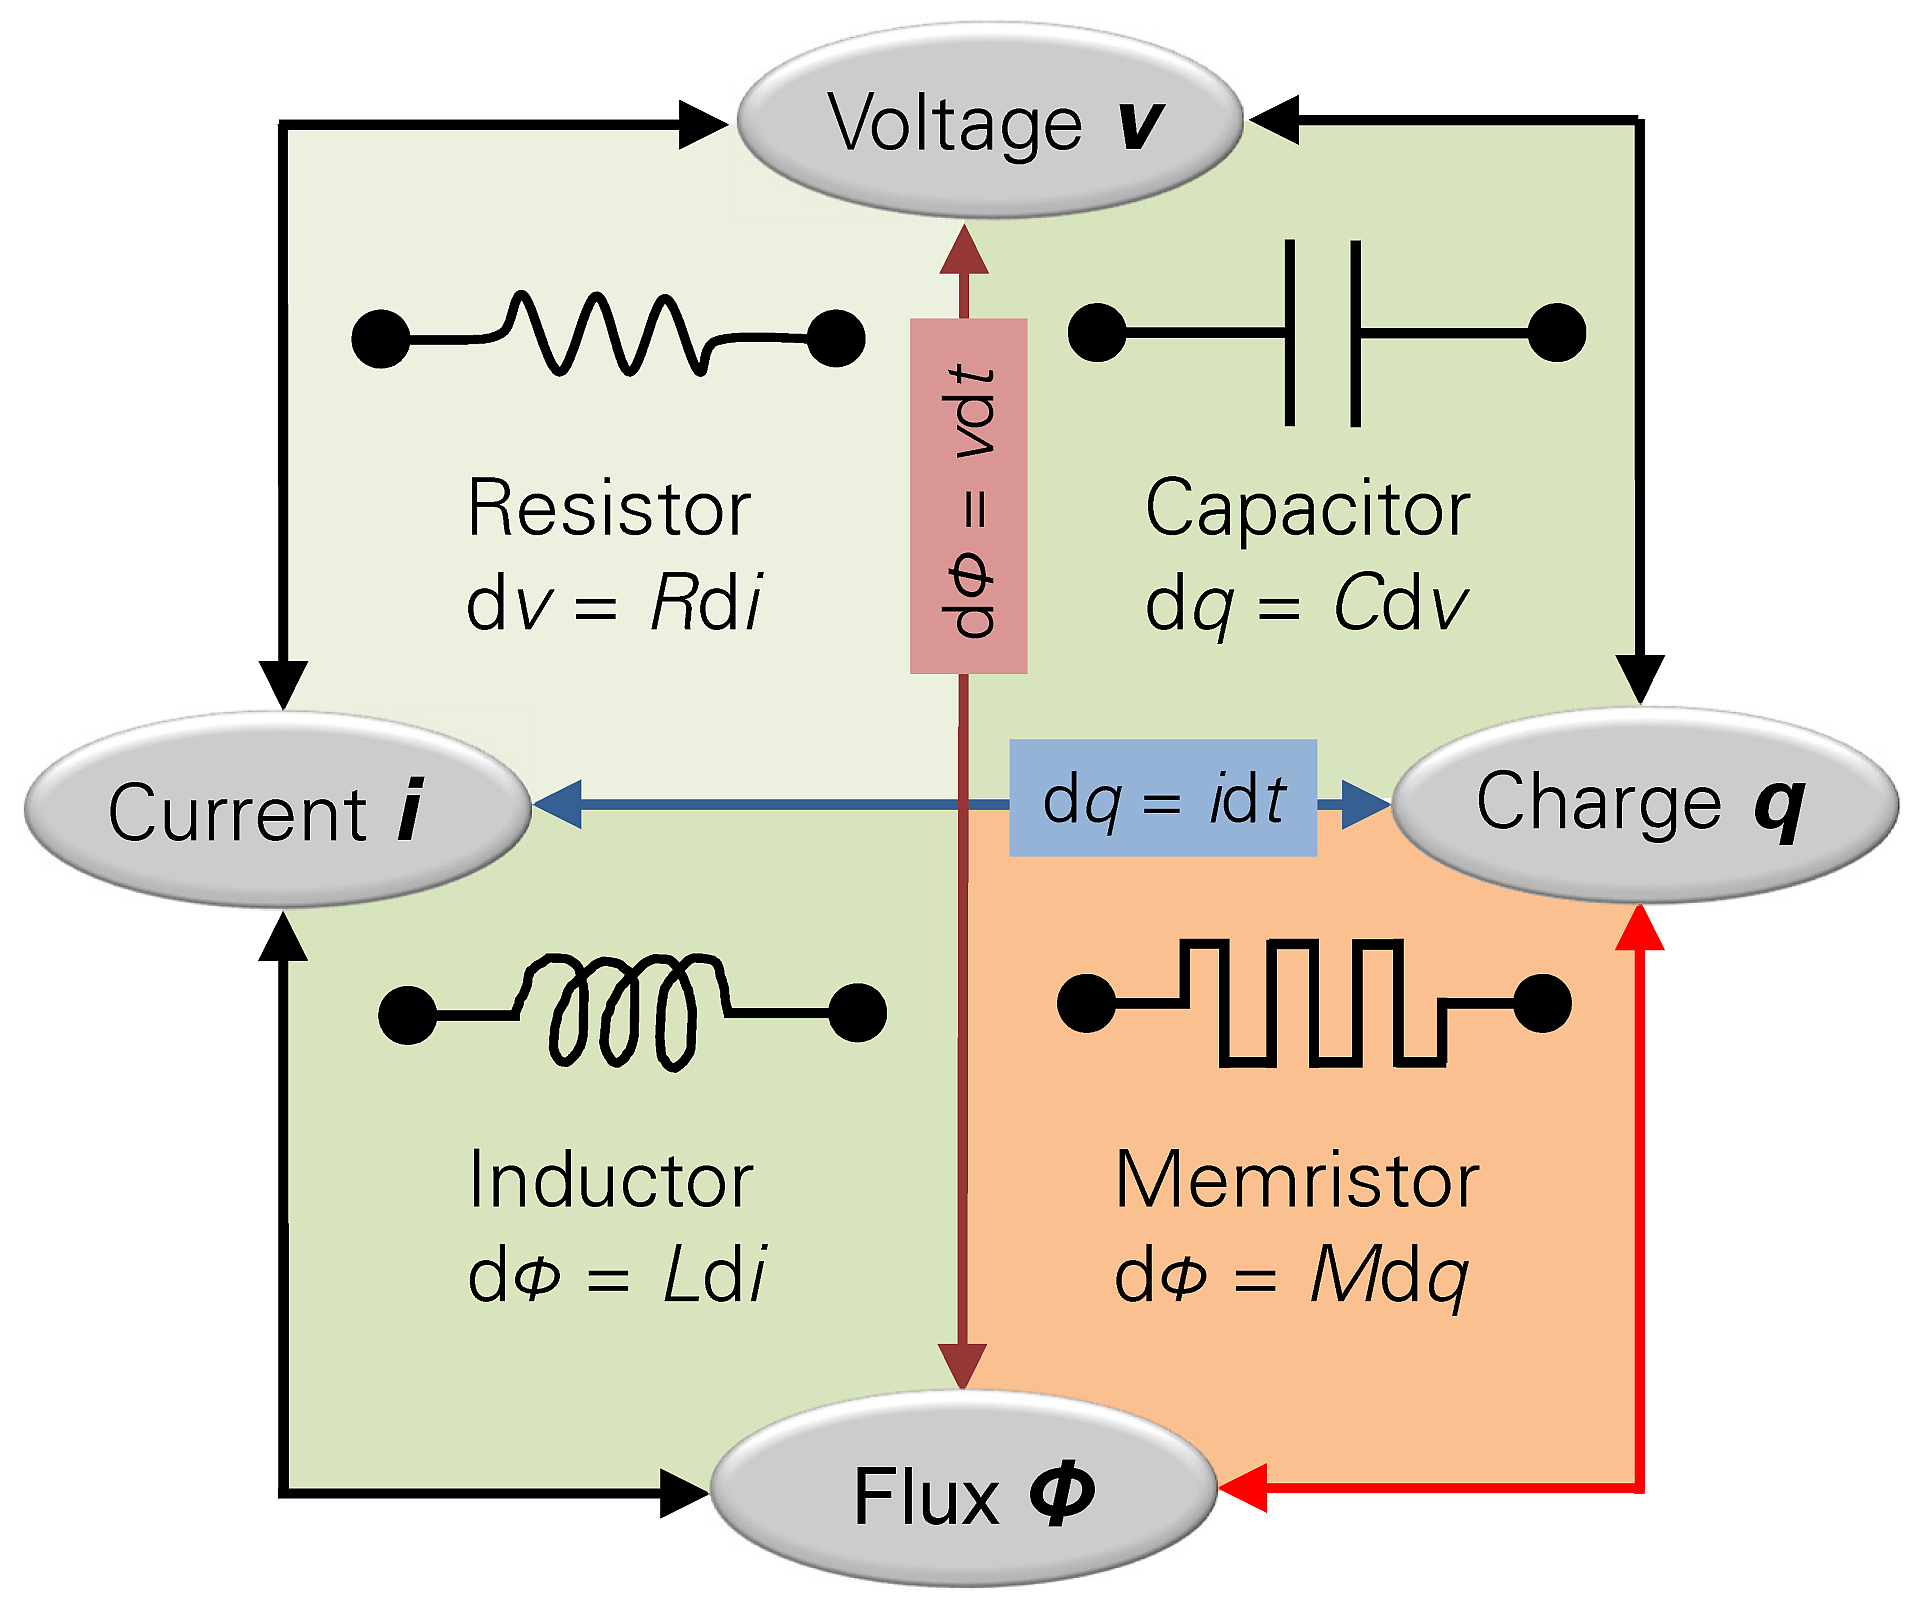
\includegraphics{memristor/memristor.png}
  \caption{Fundamental passive components}
  \label{fig:fundComp}
\end{figure}

\subsection{Equations}
A memristor links the flux ($\phi$) and charge ($q$) and creates the memristance.
This memristance is defined with the following equation :
\begin{equation}
  M(q)=\frac{d\phi}{dq}
\end{equation}
It can be compared with the other fundamental components like resistor ($R(i)=\frac{dv}{di}$), capacitor ($\frac{1}{C(q)}=\frac{dv}{dq}$) and inductor ($L(i)=\frac{d\phi}{di}$).
We can then extract a more useful equation in an actual circuit :
\begin{equation}
  v(t)=M(q(t))\cdot i(t)
\end{equation}
Similarly, a memductance can be defined as such :
\begin{equation}
  W(\phi)=\frac{dq}{d\phi}
\end{equation}
A memristive device is slightly differently defined, it still uses a memristance, but here the memristance also depends on an internal state called $x$. This gives us this equation :
\begin{equation}
  v(t)=M(x,i)\cdot i(t)
\end{equation}
The internal state ($x$) is not linked to flux or charge in the case of a memristive device.\\
Once again, we can also define the memristive device using a memductance :
\begin{equation}
  i(t)=W(x,v)\cdot v(t)
\end{equation}
In all of the previous equations, $v$ is the voltage in Volt ($V$), $i$ is the current in Ampere ($A$), $\phi$ is the flux in Weber ($Wb$), $q$ is the charge in Coulomb ($C$), $M$ is the memristance in Ohm ($\Omega$) and $W$ is the memductance in Siesmens ($S$ or $\Omega^{-1}$).

\subsection{Behavior}
A memristor is defined as a non-linear two-terminal fundamental electrical component. It behaves as a resistance with memory (hence its name), meaning that it changes its resistance based on how much charge went through it. This enables us to manipulate the resistance of the component.
The huge benefit of memristors is the memory component, when you power it, it will have the resistance it had before.

Memristive devices have a similar behavior, the memristive device's resistance will change depending on the internal state ($x$). That internal state changes based on how much and how long voltage signals or currents are applied to the memristive device.

\subsection{Usage}
The main research for memristor usage is using them as ReRAM. The idea behind ReRAM is to use memristors as Non-Volatile memory. It uses two states of the device with known resistances ($R_{on}$ and $R_{off}$), giving it binary property. Reading the memory simply requires setting a voltage and reading the output current. It is better than current solutions (HDD, SSD) as it has a much lower latency. It is better than traditionnal DRAM because it keeps the information even when turned off. This makes ReRAM a good replacement for both RAM and HDDs/SSDs, thus eliminating Von Neumann bottleneck due to the Von Neumann architecture that is used in all modern computers.

They can also be used to set a resistance to be able to perform analog multiplication. Setting them in a crossbar array makes them a very strong candidate to be used in neuromorphic computing.
